% semipy poster paper draft, 2 pages.
%
% Compiling this file needs the "svg" package to rasterize
% figures/scenario-flow.svg, which in turn needs Inkscape on PATH and
% compilation with -shell-escape, e.g.:
%
%   pdflatex -shell-escape main.tex
%   pdflatex -shell-escape main.tex   (run twice for the figure cache)
%
% If Inkscape is not available, convert the figure once by hand
% (e.g. `inkscape figures/scenario-flow.svg -o figures/scenario-flow.pdf`)
% and replace the \includesvg line below with:
%   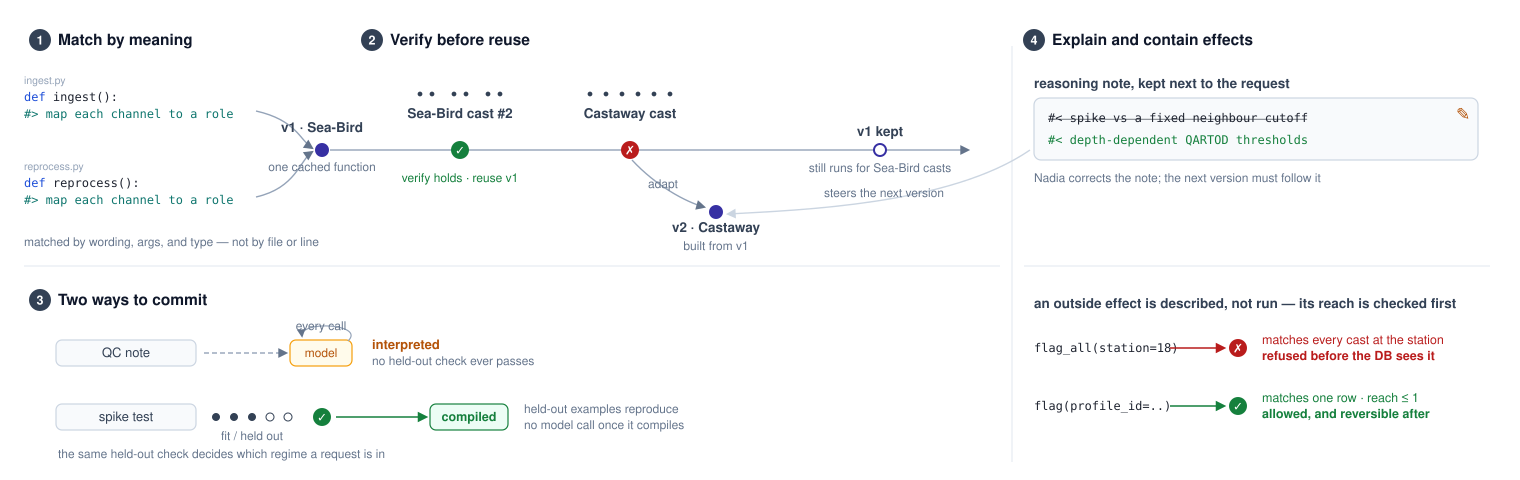
\includegraphics[width=0.98\linewidth]{figures/scenario-flow.pdf}

\documentclass[9pt]{extarticle}

\usepackage[margin=0.55in,columnsep=0.28in]{geometry}
\usepackage{times}
\usepackage{amsmath}
\usepackage{graphicx}
\usepackage{svg}
\usepackage{xcolor}
\usepackage{enumitem}
\usepackage[colorlinks=true,linkcolor=blue,citecolor=blue]{hyperref}

\setlength{\parindent}{0pt}
\setlength{\parskip}{4pt}
\setlist{leftmargin=1.1em, itemsep=2pt, topsep=2pt}

\title{\vspace{-2em}}
\date{}

\begin{document}
\pagestyle{empty}

\twocolumn[
  \begin{center}
    {\LARGE \bfseries semipy Compiles Plain-Language Requests\\
    Into Code the First Time They Run}\\[6pt]
    {\normalsize Author names withheld}\\[1pt]
    {\small Affiliation withheld}
  \end{center}
  \vspace{8pt}

  \noindent\textbf{Abstract.}\ \small
  We build semipy, a Python runtime that lets a function's behavior stay in
  plain language until the function is first called. On that first call with
  real input, semipy compiles the request into an ordinary Python function
  matched to the input it saw. Every later call rechecks that function against
  the input in front of it. semipy keeps every version it has written, and it
  checks any real-world effect a function produces before letting it run on its
  own. We explain semipy through one realistic scenario and the design
  decisions that make it work.
  \vspace{10pt}
]

\section{Introduction}

Many programs contain a small piece of logic that cannot be written
correctly until the program is actually running. A log parser has to handle
whatever format a system's log lines happen to use, and that format varies
from one deployment to the next and often changes without notice. Choosing
the right algorithm for a numerical routine depends on the shape of the data
it will actually run against, something nobody knows until the data arrives.
Turning a new, messy dataset into a clean table depends on quirks specific
to that dataset, quirks a programmer has no way to list in advance. In each
of these cases the correct behavior depends on facts that exist only once
the program is running against real input. Nothing a programmer writes down
ahead of time can capture them.

We build semipy, a Python runtime that lets a function hold a request
written in plain language in place of code written ahead of time. The first
time that request is called with real input, semipy turns it into an ordinary
Python function matched to what it saw, and that function runs from then on.
The user reads and edits the informal specification, which records the
criteria that matter for the task. The Python code underneath is generated to
meet that specification, and semipy rewrites it whenever the inputs,
invariants, or types the specification names stop matching what the current
code was built for. The user can lock the implementation at any point, and it
then stays as fixed code. A locked function needs no model, so semipy can run
inside code that executes many times a second, a rate a program could not
afford if it called a model on every input.

semipy demonstrates a way of programming in which part of a program stays an
informal specification and the code that implements it is written during real
use. We call this semi-formal programming. This paper builds the three pieces
that make it work. The first is a parser that reads an informal request
sitting inside ordinary formal code and gives the request a stable identity
from its meaning. The second is a runtime that generates a function for that
request during execution, checks it against the real input, and caches it for
later calls. The third is a way to bring the model's decisions from a run back
into the user's specification, so the user can read them and change them. The
rest of the paper walks through a realistic use of semipy and then names the
design decisions that make the runtime work this way, along with the mechanism
behind each one.

\section{Related work}

Several lines of work address parts of this problem. Systems that call a
language model on every row of data are meant for tasks whose output is open
ended, such as summarizing a document, and they accept the cost of a model
call on each row~\cite{docetl,palimpzest}. DSPy compiles a pipeline of prompts
into a fixed program whose steps are themselves prompts, so a model still runs
on each call~\cite{dspy}. semipy handles the case where a request's answer is a
fixed function of its input. It checks for that directly and calls a model
again only when a later call shows the fixed function is wrong.

Program synthesis from examples produces one program from a fixed set of
examples and uses it from then on~\cite{gulwani11}. semipy keeps each
generated function as one version in an open history and rechecks it on every
real call, opening a new version when a call contradicts it. Design by
contract checks a program against conditions a programmer writes by
hand~\cite{meyer97}. semipy records its conditions from what a generated
function actually did and checks each later revision against that record.

\section{A worked scenario}
\label{sec:scenario}

\textbf{What Nadia has and what she wants.} Nadia studies the ocean. A
research cruise has left her with a large pile of raw data files, and she
wants to turn them into clean tables that all use the same columns, the same
units, and the same meaning, so that measurements from different stops on the
cruise can be compared. Each file comes from a CTD, an instrument that the
crew lowers on a wire at each stop. As the instrument sinks and is pulled back
up, it measures the water many times a second and records temperature,
pressure, how well the water conducts electricity, how much oxygen is in it,
and more. One trip down and back up is called a cast, and each cast produces
one file.

The hard part is that every file is written differently. Two casts from the
same vendor already put their columns in a different order, report the
conductivity in a different unit, and use a different temperature scale, and a
third cast comes from another instrument that writes a comma-separated file
with full-word column names and yet another set of units. Nadia cannot write
one cleaning program in advance, because until she opens a file she does not
know which columns it has, whether a sensor drifted during the cast, or what
odd values it holds, such as a made-up number that stands for missing data or
a sudden spike from a bubble passing a sensor. What counts as a clean cast
depends on the cast in front of her. There is a second demand as well. The
same cleaning steps have to run later on their own, first over the cruise's
hundreds of casts, then over millions of older casts in an archive, and
eventually on small robots that drift in the ocean for weeks with no internet.
Asking a large model about every single measurement would be far too slow, and
the robots cannot reach a model at all, so the finished cleaning steps have to
be plain, fast Python code that runs by itself.

\begin{figure*}[t]
  \centering
  \includesvg[width=0.98\linewidth]{figures/scenario-flow}
  \caption{One request's life inside semipy, following Nadia's cruise, read
  left to right. Step 1 recognizes a request written the same way at two call
  sites, her live ingest and her end-of-day reprocessing pass, and reuses one
  cached function for both. Step 2 checks that reuse against a real cast before
  trusting it, and a failure opens a new version while the one that already
  works stays in place. Step 3 shows two ways to commit. A request with no
  stable function keeps running through the model, and a rule-based request
  compiles into code once a held-out check passes. Step 4 shows a reasoning
  note edited by hand and a real effect checked against the database schema
  before it is allowed to run on its own.}
  \label{fig:flow}
\end{figure*}

\textbf{Leaving the changeable part as a sentence.} semipy lets Nadia leave
the part she cannot write yet as a plain sentence sitting inside an otherwise
normal Python function. Her first job is to work out which column of a file is
the temperature, which is the pressure, and so on, and this is exactly the
part that changes from file to file. She writes a normal function that
receives the column names and units read from one file and is declared to
return a dictionary that pairs each column with one standard name. Where the
body of the function would normally go, she writes one English sentence marked
with \verb|#>| and leaves the result unfilled.

\begin{verbatim}
@semiformal
def map_channels(names, units) -> dict[str, str]:
    #> map each column to one standard role,
    #> using the units to tell them apart
    roles = ...
    return roles
\end{verbatim}

The sentence after \verb|#>| is the informal part, and it says what Nadia
wants. The code around it is the formal part, and it fixes what the answer is
allowed to be. The function is handed only the names and units, so the answer
can look at nothing else. The list of standard roles is fixed elsewhere in her
code, so the answer may use only those roles. The return type says the answer
has to be a dictionary. Nadia never writes the body herself. The first time
this function runs on a real file, semipy reads her sentence together with the
code around it, asks a model to write the missing Python, runs that Python on
the actual file, and checks that the result is a dictionary of allowed roles.
From then on the generated function is what runs, and no model is called again
unless a later file breaks it. Every changeable step in her pipeline is
written this way, as one sentence fenced in by the formal code that feeds it
and the formal code that uses its answer.

\textbf{The same sentence in two scripts becomes one function.} Nadia runs two
scripts. One cleans casts as they come off the wire during the cruise, and the
other reprocesses the whole day's casts together overnight. She writes the
same \verb|map_channels| sentence in both. semipy treats two requests as the
same when their sentence, the variables they read, and their return type all
match, and it pays no attention to which file or line they sit on. The two
copies match, so semipy writes the function once and both scripts call it
(Figure~\ref{fig:flow}, step 1). That one function goes on to map the columns
for every instrument on the cruise.

\textbf{Every reuse is checked against the real file.} A second sentence, in a
function called \verb|downcast_indices|, keeps only the part of a cast where
the instrument is steadily sinking and throws away the readings from when it
still sat near the surface and from the trip back up. semipy writes this
function on the first cast, which is a deep one. When a second deep cast
arrives, semipy does not simply reuse the function. It runs the existing
function on the new cast and checks the result first, because code that worked
on one cast can still be wrong on the next. The check passes, so the function
is reused. Then a shallow cast only eight meters deep arrives from the third
instrument, and the same function fails the check, because the long steady
descent it was written to find is not there. semipy writes a new version for
the shallow case and keeps the old version untouched (Figure~\ref{fig:flow},
step 2), so fixing the shallow casts cannot break the deep casts that already
work.

\textbf{Some sentences turn into code and some keep calling a model.} A
sentence turns into code only when one fixed function can answer it. Alongside
the cleaning steps, Nadia wants a short QC note for each cast, which is one
plain sentence written for a human reviewer that says what to look at, for
example that a sensor reads suspiciously. The right note changes from cast to
cast and no single fixed function can produce it, so Nadia marks that sentence
as interpreted, which tells semipy to call a model for it on every run and
never try to turn it into code. A different sentence, a standard test that
flags a temperature reading sitting too far from the average of its two
neighbors, does follow a fixed rule. For a sentence like this semipy writes a
candidate function from most of a small set of real casts, holds a few casts
back, and checks whether the function reproduces the ones it held back. Once
it does, the sentence becomes ordinary compiled code (Figure~\ref{fig:flow},
step 3). That code then runs with no model and no network, which is what lets
it run over millions of archived casts and on a robot at sea.

\textbf{Reading a decision, correcting it, and fencing in real changes.} Each
time semipy writes or rewrites a function, it also writes a short note next to
the sentence saying how that function decides. For the spike test the note
explains that the function compares each reading to the average of its two
neighbors and flags it when the gap is larger than a set cutoff. Nadia knows
her region uses a cutoff that changes with depth, so she edits the note to say
so, and semipy writes the next version to match her correction
(Figure~\ref{fig:flow}, step 4). One kind of step reaches outside the program,
such as writing a quality flag into the shared cruise database that the whole
team reads. semipy never lets a generated function write to that database
itself. The function only returns a description of the change it wants, and
semipy checks that description against a plain rule before anything happens.
The rule is that the change may touch only one named cast and never a whole
group of casts. When a sentence would have flagged every cast in the table at
once, semipy refuses it before the database is touched (Figure~\ref{fig:flow},
step 4).

\textbf{Seeing and steering all of this in the editor.} Nadia does everything
above from the semipy extension for VS Code, which shows each step inside her
editor and lets her act on it (Figure~\ref{fig:vscode}). When she runs the
ingest script, a one-line summary appears above each of these functions, for
example \texttt{GENERATE\ $\cdot$\ verified\ $\cdot$\ maps 6 channels}, and
clicking it opens the full detail. On the binning step, semipy could not decide
how to handle a depth range that holds only missing values, so it shows the
choice in the editor as a line marked \verb|#?| along with the real input and
output of each option. Nadia clicks the option she wants, and the running
function switches to it with no model call. On the spike test she promotes her
corrected note from a \verb|#<| note line into a \verb|#>| request line with
one click, which makes her depth-based cutoff a permanent part of what the
sentence asks for. When the shallow cast created a second version of
\verb|downcast_indices|, the marker on it reads \texttt{v1/2}. She clicks the
marker, opens the first version to confirm it still runs on a deep cast, and
then returns to the newest one. Throughout, a split view keeps the generated
code next to her own source, shown dimmed until she edits a line herself.

\begin{figure}[t]
  \centering
  % TODO: replace this placeholder with a real screenshot of the semipy VS
  % Code extension showing the CodeLens health sentence, a #? fork picker,
  % a promoted #< -> #> line, and the v1/2 version checkout on downcast_indices.
  \setlength{\fboxsep}{0pt}%
  \fbox{\parbox[c][3.9cm][c]{0.96\linewidth}{\centering\small\itshape
    \color{gray} screenshot of the semipy VS Code extension:\\
    one-line summary, the \texttt{\#?} picker on \texttt{bin\_1dbar},\\
    a promoted \texttt{\#<}\,$\to$\,\texttt{\#>} threshold on the spike test,\\
    and the \texttt{v1/2} checkout on \texttt{downcast\_indices}\\[2pt]
    (to be added)}}
  \caption{The editor shows each step: the decision as a one-line summary, a
  silent choice as a \texttt{\#?} picker, a corrected note promoted from
  \texttt{\#<} to \texttt{\#>}, and every saved version reachable by checkout.}
  \label{fig:vscode}
\end{figure}

\section{Design guidelines}

\textbf{A request's identity comes from its meaning.} semipy computes three
identifiers for a request. Let $s$ be a request's wording, with free
variables $\mathrm{args}(s)$ in order, declared return type $\mathrm{type}(s)$,
the kind of code region it sits in $\mathrm{cat}(s)$, and its named outputs
$\mathrm{out}(s)$. The meaning key
\[
k(s) = \mathrm{hash}\big(\mathrm{template}(s), \mathrm{args}(s),
\mathrm{type}(s), \mathrm{cat}(s), \mathrm{out}(s)\big)
\]
leaves out the file, the line, and the runtime values. Two requests at
different call sites with the same $k(s)$ can share one function, which is how
the reprocessing pass reused the channel map written by the live ingest. A
second identifier, keyed on the exact wording and call site, tracks one
request's own version history, so editing the wording on purpose starts a
fresh history.

\textbf{Reuse is checked against the real call before it is trusted.} Given a
candidate function $f$ and the current call's real arguments $x$, semipy
reuses $f$ only when $\mathrm{verify}(f, x)$ holds. When it fails and $f$
already has a version history, semipy adapts a new version from $f$. When the
request nearly matches an earlier one with a single part swapped, semipy fills
in that pattern directly with no model call. Otherwise it generates a new
function with a model. semipy checks every one of these outcomes against $x$
before trusting it, which is why the shallow Castaway cast produced a checked
failure and a new version rather than a wrong profile in the database.

\textbf{Committing to code waits for evidence and can always be revised.}
Every accepted function is one commit in a per-request version history, and
nothing is deleted, so the active function is the newest commit across every
open version. A request marked \texttt{interpreted} answers each call with a
model, holds out about a third of the examples it has seen, and compiles into
a fixed function once a function written from the rest reproduces every
held-out example. When that never happens, semipy keeps calling the model.
After a request compiles, running it costs an ordinary function call, far
below what an interpreted call costs, which is a full round trip to a model.
The same held-out check decides which of the two regimes a request is in.

\textbf{The user steers the specification through what the runtime surfaces.}
After each generation semipy writes a short reasoning note next to the request
describing how the current function decides. When the model had to choose
between two readings of the request that would behave differently, semipy
records that fork and shows it inline with the input and output of each
branch. The user resolves the fork by picking a branch, which swaps the
active function with no model call, or by stating a property the answer must
satisfy, which drives the next generation. Editing the reasoning note steers
the next version the same way, and promoting the note into the request text
makes the correction a permanent part of what the request means. Because every
accepted function stays in the version history, the user can check out an
earlier version at any time and return to the newest one afterward. Each of
these actions is an edit to the specification, and the runtime answers it by
reusing, adapting, or regenerating the code underneath.

\textbf{Real effects are described and checked before they run.} A generated
function that reaches outside the program returns a description of the change
it wants and never touches real state directly. semipy checks that description
against two properties before anything happens. The change must be reversible,
and its reach must be provably bounded. When a target table has a column that
is unique per row, a key $K$, and a change's condition pins one value of $K$,
then for any input,
\[
\forall\, x.\ \ \mathrm{condition}(x) \Rightarrow
|\{\text{rows matched}\}| \le 1,
\]
checked from the schema with no model call. This caught the request that would
have flagged every cast in the table instead of the one cast in front of it.

\section{Closing}

Three extensions follow from the current limits of the system. A request is
always captured as text today, though the meaning key and the decision
procedure work the same whatever the request is made of. The same matching and
versioning could apply to a request given as a short audio clip, a sketch, or
a recorded gesture, wherever that is the clearer way to say what is wanted.
Some requests stay in interpreted mode because no fixed Python function
reproduces their held-out examples. The same held-out check could accept a
small trained model as the promotion target, so a request that no fixed
function fits can still settle into a cheaper, faster answer. The conditions
semipy records today come from what a generated function actually did.
Recording properties that a programmer states once in plain language, and
checking every future revision against them, would let the programmer write a
contract once and have the runtime enforce it on its own.

{\small
\begin{thebibliography}{9}

\bibitem{docetl} S. Shankar, T. Chen, et al. DocETL: agentic query rewriting
and evaluation for complex document processing. 2024.

\bibitem{palimpzest} C. Liu, M. Russo, et al. Palimpzest: optimizing
AI-powered analytics with declarative query processing. CIDR 2025.

\bibitem{dspy} O. Khattab, A. Singhvi, et al. DSPy: compiling declarative
language model calls into self-improving pipelines. ICLR 2024.

\bibitem{gulwani11} S. Gulwani. Automating string processing in spreadsheets
using input-output examples. POPL 2011.

\bibitem{meyer97} B. Meyer. Object-Oriented Software Construction, 2nd
edition. Prentice Hall, 1997.

\end{thebibliography}
}

\end{document}
